\documentclass[a11paper]{article}
% xelatex

\usepackage{subcaption}
\usepackage{tabularx}
\usepackage{libs/titlepage}
\usepackage{libs/document}
\usepackage{booktabs}
\usepackage{multicol}
\usepackage{multirow}
\usepackage{float}
\usepackage{varwidth}
\usepackage{graphicx}
\usepackage{siunitx}
\usepackage{pifont}
\usepackage{subcaption}
% \usepackage[toc,page]{appendix}
\usepackage[usenames,dvipsnames]{xcolor}

\title{Rapport d'APP}

\class{Logique Combinatoire}
\classnb{GEN420 \& GEN430}

\teacher{Berthié Gouin-Ferland \& Nikola Zelovic}

\author{
  \addtolength{\tabcolsep}{-0.4em}
  \begin{tabular}{rcl} % Ajouter des auteurs au besoin
      Benjamin Chausse & -- & CHAB1704 \\
      Shawn Couture    & -- & COUS1912 \\
  \end{tabular}
}

\newcommand{\todo}[1]{\begin{color}{Red}\textbf{TODO:} #1\end{color}}
\newcommand{\note}[1]{\begin{color}{Orange}\textbf{NOTE:} #1\end{color}}
\newcommand{\fixme}[1]{\begin{color}{Fuchsia}\textbf{FIXME:} #1\end{color}}
\newcommand{\question}[1]{\begin{color}{ForestGreen}\textbf{QUESTION:} #1\end{color}}

% Checkboxes
\setlength{\fboxsep}{1pt}
\newcommand{\cbox}{\fbox{\phantom{\ding{51}}}}
\newcommand{\cboxtick}{\fbox{\ding{51}}}%

\newcommand{\quicktable}[4]{
  \begin{table}[H]
    \footnotesize
    \centering
    \caption{#1}
    \label{tab:#2}
    \begin{tabular}{#3}
      #4
    \end{tabular}
  \end{table}
}

\newcommand{\quickfigure}[4]{
  \begin{figure}[H]
    \centering
		\includegraphics[width=#3\textwidth]{#4}
    \caption{#1}
    \label{fig:#2}
  \end{figure}
}

\begin{document}
\maketitle
\newpage
\tableofcontents
\listoffigures
\listoftables
\newpage

% \note{Un total de 4 pages est permis, excluant la page titre, la table des matières, l'introduction,
% la conclusion et les références.}

\section{Introduction}

Dans le cadre de l'APP2 de la session S4, il est demandé de compléter le
développement d'une pédale d'effets de guitare numérique à l'aide d'un FPGA
sur la carte Zybo. Plus précisément, ce rapport documente la conception,
l'implémentation et la vérification de deux modules essentiels au système:
le décodeur I2S (M1), responsable de la désérialisation du signal audio reçu,
et le module de calcul de la puissance du signal (M6). Ces travaux ont été
réalisés en respectant les contraintes de synchronisation, de modularité et
de formalisme en VHDL, selon les normes enseignées. Le rapport présente les
diagrammes d'états, les schémas-blocs, les plans de vérification ainsi que
les résultats de simulation attestant de la conformité fonctionnelle des
modules développés.

\section{Module M1}

% \note{votre lecteur ne connait pas votre démarche ni
% pourquoi un tel résultat démontre le bon fonctionnement – vous devez l'expliquez brièvement.}

% \note{Nous ne consulterons pas le dépôt de vos fichiers Xilinx (sauf
% dans des cas particuliers) ce qui signifie que votre rapport doit être complet en lui-même.}

\subsection{Description du fonctionnement}

Le décodeur I2S détecte et extrait les échantillons stéréo (gauche et droite)
transmis en série par le CODEC audio via le protocole I2S. Son
fonctionnement repose sur une machine à états finis synchronisée par
l'horloge bit \verb|i_bclk|.\\

\quickfigure{Machine à états finis du module M1}{mef-m1}{}{figures/m1-mef-mermaid.pdf}

Le module débute dans l'état \verb|awaiting_lrc_front_change|, où il détecte
une transition sur le signal de sélection de mot \verb|i_lrc|. Lorsqu'une transition
est détectée, le compteur de bits et le registre à décalage sont réinitialisés,
et l'état passe à \verb|reading_24bit_word|.\\

Dans cet état, les bits sont captés en série à chaque front d'horloge et
décalés dans un registre. Une fois 23 bits reçus (le bit 0 étant le premier),
le décodeur passe à l'état \verb|saving_received_word|, où il déclenche le chargement
du mot complet dans un registre parallèle : vers \verb|o_load_left| si le mot
correspond au canal gauche (\verb|i_lrc| = 0), ou vers \verb|o_load_right| si
c'est le canal droit (\verb|i_lrc| = 1).\\

Finalement, l'état bascule à \verb|setting_str_dat| et active le signal \verb|o_str_dat| si le mot
appartient au canal droit. Ce signal sert à synchroniser les modules en aval,
comme les fonctions de calcul de puissance et de fréquence, qui ne s'appuient
que sur les échantillons du canal droit. Le système revient ensuite à l'attente
d'une nouvelle transition sur \verb|i_lrc|.\\

\subsection{Validation et vérification}

\quicktable{Plan de vérification du module M1 -- décodeur I2S}{mef-m1}{p{4cm}p{5cm}p{6cm}l}{

  \toprule
  \textbf{Objectif Ciblé} & & \textbf{Valider la MEF décodeur I2S} & \\
  Condition à proscrire & Aucune & & \\
  \midrule
  \textbf{Test} & \textbf{Action} & \textbf{Résultat attendus} & \cboxtick \\
  \midrule

  Condition initiale
  & Aucune
  & Les registres et échantillons sont à $0$.
  & \cbox \\

  Reset initial
  & \texttt{BTN3} à $1$
  & Les registres restent à $0$ peut importe la valeur des échantillons.
  & \cbox \\

  Envoie répétitif du même code au même channel. (droite)
  & Envoie de 4x \texttt{0xF0F0F0} au channel droit (.txt)
  & \texttt{0xF0F0F0} est lu sur le registre de droit pour la durée de 4 affichages.
  & \cbox \\

  Envoie répétitif du même code au même channel. (gauche)
  & Envoie de 4x \texttt{0xF0F0F0} au channel gauche (.txt)
  & \texttt{0xF0F0F0} est lu sur le registre de gauche pour la durée de 4 affichages.
  & \cbox \\

  Test de messages mix (droite)
  & Envoie de suites d'ondes à fréquences qui augmentent au channel droit (.txt)
  & Les échantillons sont présentés à la sortie du registre de droit sans changement.
  & \cbox \\

  Test de messages mix (gauche)
  & Envoie de suites d'ondes à puissances qui augmentent au channel gauche (.txt)
  & Les échantillons sont présentés à la sortie du registre de gauche sans changement.
  & \cbox \\

  Test de reset en pleine lecture
  & Envoie d'onde constantes aux deux channels, appui sur BTN3 en pleine lecture.
  & Les sorties des registres tombent à 0. La lecture recommence lorsque \texttt{LRC} change de front.
  & \cbox \\

\bottomrule
}

Les chronogrammes fournis ont été fait à l'aide du banc de test fourni. Quelques noms de certains signaux ont été changés afin d'être intuitif.
\ref{fig:chrono-m1-param-enable-reg-activation-return-await} démontre l'activation du bon registre \verb|o_load_right| si \verb|lrc| est à $1$ et le tout dans les bons états (jaune).
\ref{fig:chrono-m1-detect-change-LRC-save-output-to-channel} démontre à l'aide de curseur les moments précis ou la lecture sur 24 bits est effectués.
Autrement dit, un cycle complet de la machine à états. Ont voit le changement de LRC et la lecture qui commence une monté d'horloge plus loin.
\ref{fig:chrono-m1-input-becomes-output} démontre que les signaux qui sorte du décodeur sont les mêmes que les signaux qui entre dans le banc de test.
Le décalage des ondes s'explique par le fait qu'elles doivent passé dans le codeur avant le décodeur et ces exécutions prennent plusieurs coup d'horloge de délai.
Finalement, la figure \ref{fig:chrono-m1-reset-works-awaits-LRC-change} démontre le fonctionnement du reset. Tout est à zéro temps que le bouton est appuyé et
la lecture recommence uniquement lors du changement de LRC après l'arrêt du signal de reset.

\begin{figure}[H]
  \centering
  \begin{subfigure}{.496\linewidth}
    \centering
    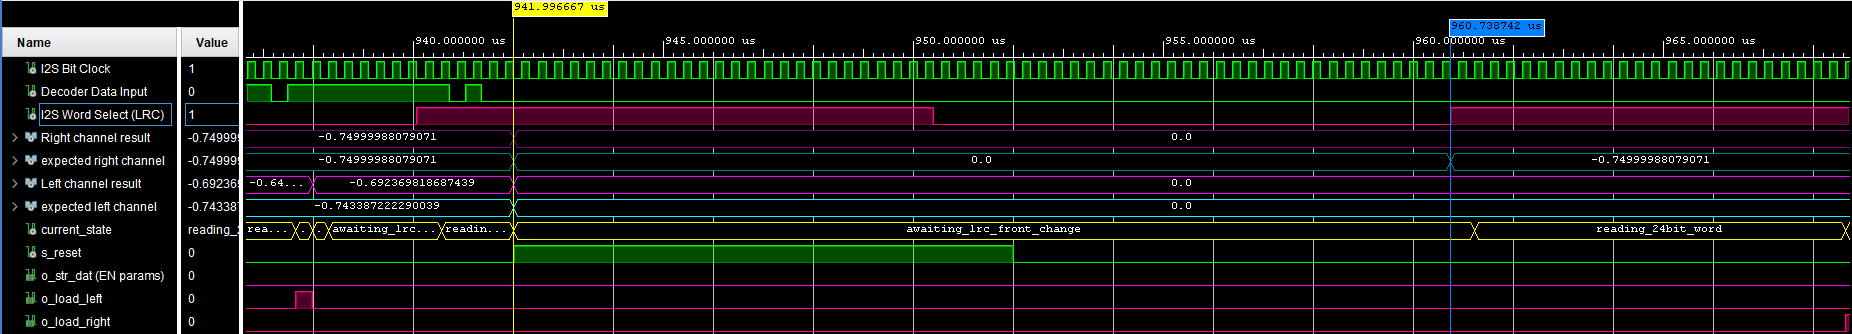
\includegraphics[width=\textwidth]{figures/chrono-m1-reset-works-awaits-LRC-change.png}
    \caption{Fonctionnement du reset et attente du changement de LRC}
    \label{fig:chrono-m1-reset-works-awaits-LRC-change}
  \end{subfigure}
  \begin{subfigure}{.496\linewidth}
    \centering
    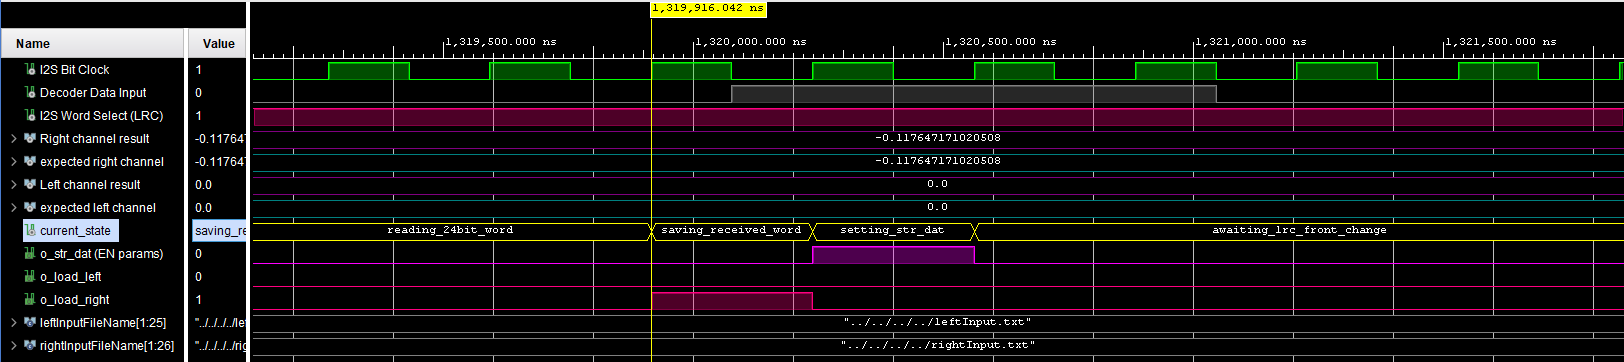
\includegraphics[width=\textwidth]{figures/chrono-m1-param-enable-reg-activation-return-await.png}
    \caption{Activation des registres et retour à l'état d'attente}
    \label{fig:chrono-m1-param-enable-reg-activation-return-await}
  \end{subfigure}
  \begin{subfigure}{.496\linewidth}
    \centering
    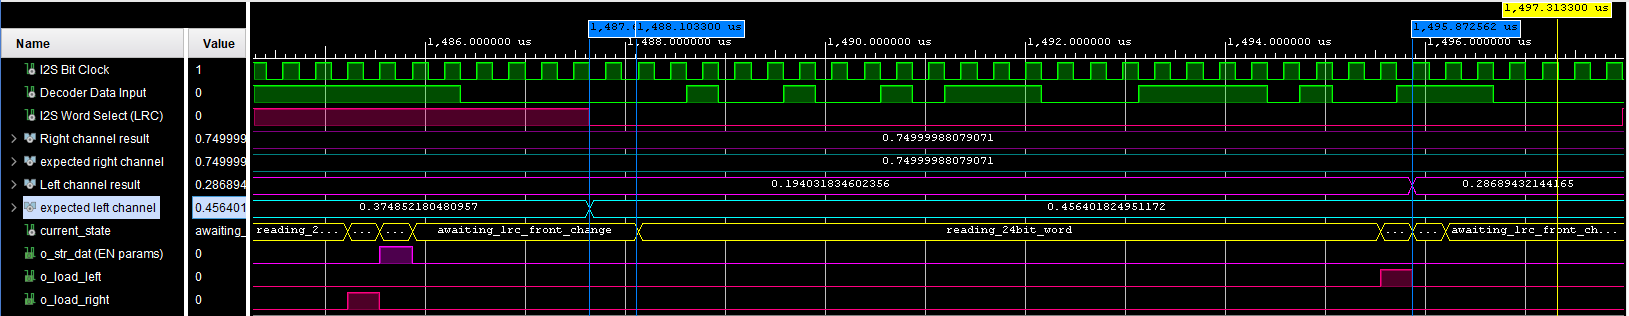
\includegraphics[width=\textwidth]{figures/chrono-m1-detect-change-LRC-save-output-to-channel.png}
    \caption{Détection du changement de LRC et enregistrement des données dans le canal approprié}
    \label{fig:chrono-m1-detect-change-LRC-save-output-to-channel}
  \end{subfigure}
  \begin{subfigure}{.496\linewidth}
    \centering
    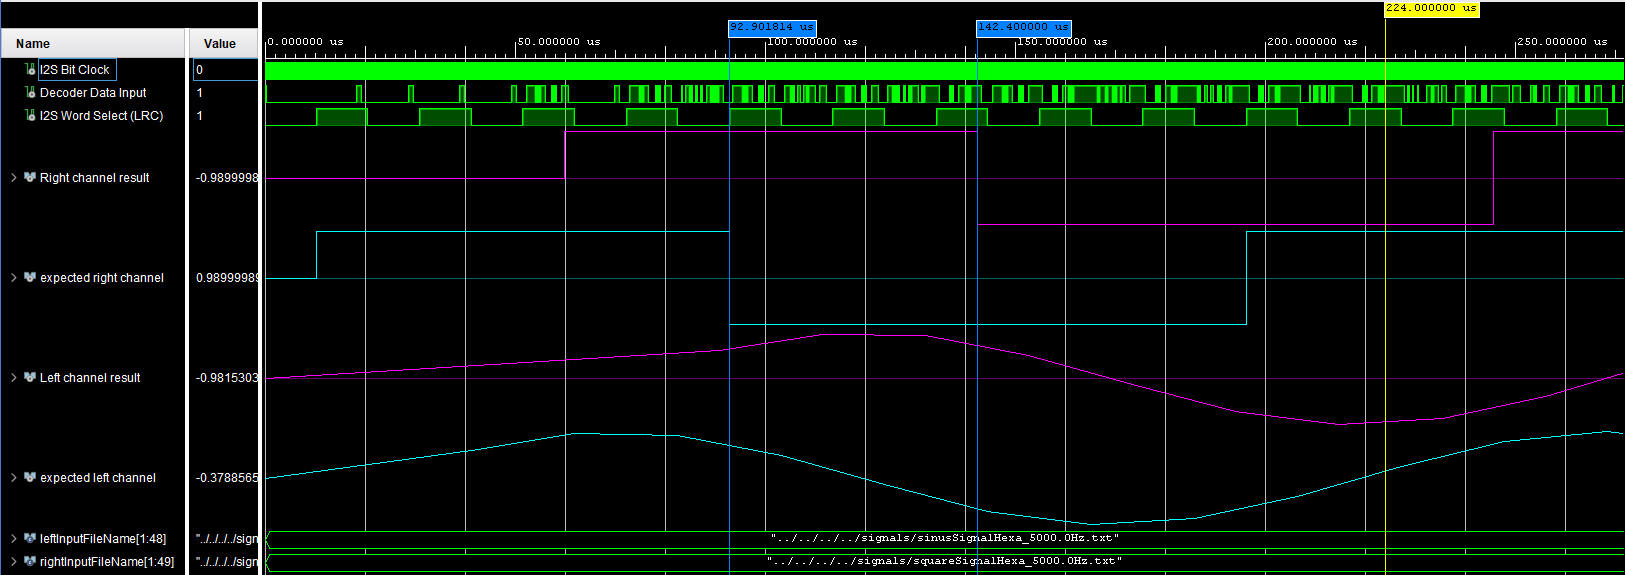
\includegraphics[width=\textwidth]{figures/chrono-m1-input-becomes-output.png}
    \caption{Conversion des données de sérial en entrée à parallèle en sortie}
    \label{fig:chrono-m1-input-becomes-output}
  \end{subfigure}
  \caption{Chronographes du module M1 sous différentes conditions}
\end{figure}

% \todo{Validation via une simulation avec le banc de test fourni. Vous devez démontrer le
% fonctionnement de vos modules au travers de simulations et expliquez en quoi vous
% répondez aux spécifications. Faites bon usage des curseurs, formattage des données et
% agrandissements pour appuyer vos propos.}

\section{Module M6}

% \note{votre lecteur ne connait pas votre démarche ni
% pourquoi un tel résultat démontre le bon fonctionnement – vous devez l'expliquez brièvement.}

% \note{Nous ne consulterons pas le dépôt de vos fichiers Xilinx (sauf
% dans des cas particuliers) ce qui signifie que votre rapport doit être complet en lui-même.}

\subsection{Description du fonctionnement}


% \quickfigure{Machine à états finis du module M6}{mef-m6}{}{figures/m6-mef-mermaid.pdf}

% \todo{Schéma-bloc du système}

Le module M6 effectue une estimation de la puissance du signal audio en
appliquant un filtrage exponentiel à moyenne glissante sur les échantillons
entrants. Le calcul s'effectue à chaque front montant de l'horloge
\verb|i_bclk|, lorsque le signal \verb|i_en| est à 1. \\

\quickfigure{Schéma bloc du module M6}{m6-bloc}{.75}{figures/blok-drawio.pdf}

À chaque activation, la puissance instantanée est calculée en élevant au
carré l'échantillon courant \verb|i_ech|. Cette nouvelle valeur est ensuite
ajoutée à l'historique de puissance, qui est préalablement réduite par un
facteur d'oubli de 31/32. Ce facteur assure que les résultats récents ont
plus de poids que les anciens, tout en limitant la croissance de la valeur
accumulée afin d'éviter un débordement (\emph{overflow}). \\

Le résultat final est stocké dans le registre \verb|oldest_power|. Pour
simplifier l'affichage ou l'utilisation de cette puissance, seuls les bits de
poids fort (\verb|oldest_power(46 downto 39)|) sont extraits et envoyés sur
la sortie \verb|o_param|. \\

\subsection{Vérification et validation}

\quicktable{Plan de vérification du module M6 -- Calcul de puissance}{mef-m6}{p{4cm}p{5cm}p{6cm}l}{
  \toprule
  \textbf{Objectif Ciblé} &
  & \multirow{2}{*}{\textbf{Valider la MEF calcul de puissance d'ondes}}
  & \\
  Condition à proscrire
  & Ondes ayant une fréquence plus haute que \SI{24}{\kilo\hertz}
  &
  & \\
  \midrule
  \textbf{Test}
  & \textbf{Action}
  & \textbf{Résultat attendus}
  & \cboxtick \\
  \midrule
  Condition initial
  & Mettre les interrupteurs à 0010 et une onde sans amplitude
  & La puissance en sortie reste à 0.
  & \cbox\\
  Reset initial
  & \texttt{BTN3} à 1 et onde sans amplitude.
  & La valeur de la puissance devient 0 et reste à 0 après.
  & \cbox\\
  Test d'une onde sinuosïdale
  & Mettre une onde sinus de \SI{1}{\kilo\hertz}. À amplitude maximum
  & La puissance augmente et oscille en suivant l'amplitude du signal d'entrée
  & \cbox\\
  Test d'une onde sinusoïdale avec bruit
  & Mettre une onde sinus de \SI{1}{\kilo\hertz} avec un peu de bruit. À amplitude maximum
  & La puissance augmente et oscille a la même fréquence que le signal d'entrée. Observation d'atténuation du bruit.
  & \cbox\\
  Test d'une onde Carré
  & Mettre une onde carré de \SI{1}{\kilo\hertz} à amplitude maximum
  & La puissance augmente vers le maximum et reste stable.
  & \cbox\\
  Test de haute fréquences
  & Mettre une onde sinus de \SI{20}{\kilo\hertz}
  & La puissance oscille en fonction de l'amplitude du signal. la valeur de la puissance reste en moyenne plus haute que l'onde de \SI{1000}{\hertz} (à cause de l'accumulation).
  & \cbox\\
  Test de saturation
  & Un signal d'amplitude maximum envoyé en continue
  & La puissance atteint le maximum après quelques échantillons et aucun débordement se produit.
  & \cbox\\
  Test d'amplitude fix basse
  & Onde carrée d'amplitude 0.5 à -0.5 envoyé en entrée
  & la puissance atteint la moitié du maximum après quelques échantillons et reste stable
  & \cbox\\
  \bottomrule
}

Le fonctionnement réponds plus ou moins aux spécifications.
À cause de la méthode utilisé, la mesure de la puissance ne se stabilise pas assez lentement pour donner un nombre fixes
à des basses fréquences (\ref{fig:chrono-m6-1000hz-sin-noisy}). Cependant ce chronogramme démontre la résistance au bruit.
La figure \ref{fig:chrono-m6-reset-and-20000hz} démontre le bon fonctionnement du reset (le tout reste à zéro jusqu’à la relâche du signal en rouge).
La figure \ref{fig:chrono-m6-saturation-works} démontre que le calcul monte tranquillement vers le maximum (prouvant l'utilisation d'accumulation)
et n'éprouve aucun dépassement restant stable. la figure \ref{fig:chrono-m6-square-5000hz-2in1} démontre que la puissance reste stable et s'adapte
aux changements d'amplitude du signal entrant dans le module. le chronogramme \ref{fig:chrono-m6-reset-and-20000hz} à une sinus à l'entrée, mais le graphique
à été réalisé avec la fonction d'affichage « hold » se qui donne l'impression d'une onde carré. Les spécification sont
donc atteinte car un facteur de 31/32 est utilisée et une accumulation en continue est présente. Cependant, l'angle d'approche
serait à revoir afin d'avoir des lectures stables avec des ondes sinusoïdales.


\begin{figure}[H]
  \centering
  \begin{subfigure}{.496\linewidth}
    \centering
    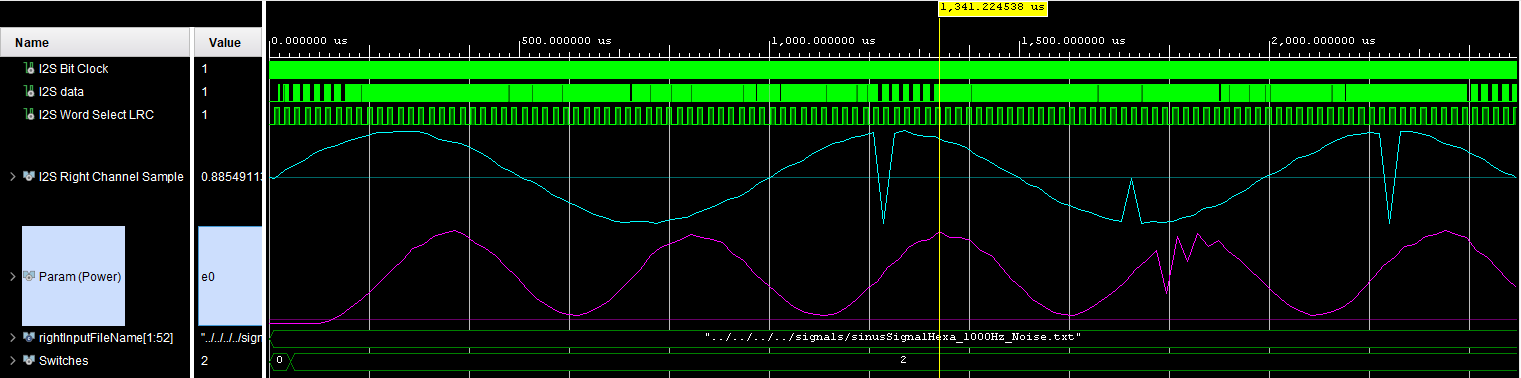
\includegraphics[width=\textwidth]{figures/chrono-m6-1000hz-sin-noisy.png}
    \caption{Signal sinusoïdal bruité à \SI{1}{\kilo\hertz}}
    \label{fig:chrono-m6-1000hz-sin-noisy}
  \end{subfigure}
  \begin{subfigure}{.496\linewidth}
    \centering
    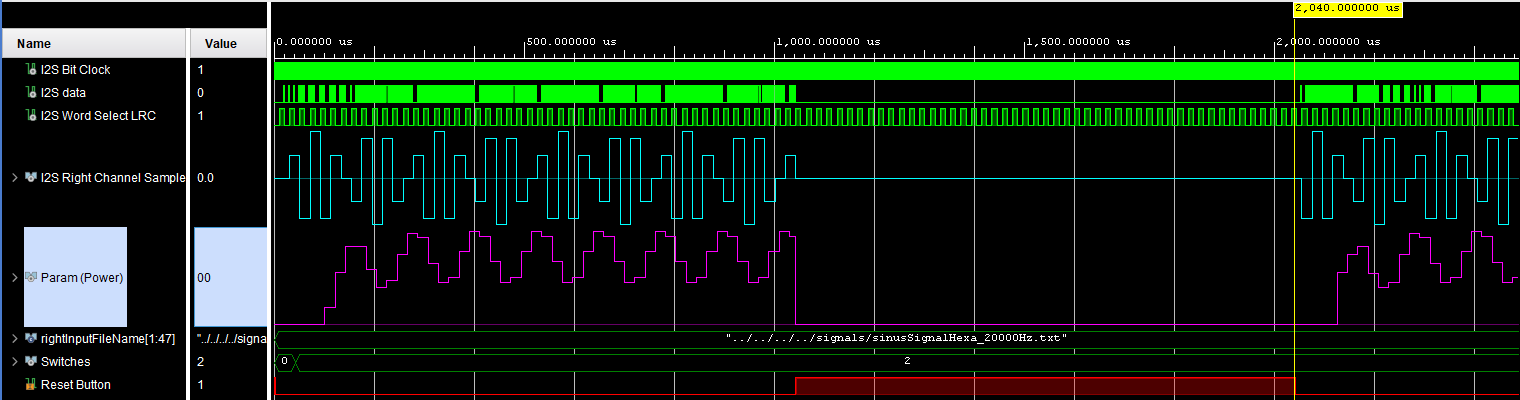
\includegraphics[width=\textwidth]{figures/chrono-m6-reset-and-20000hz.png}
    \caption{Post-réinitialisation et signal à \SI{20}{\kilo\hertz}}
    \label{fig:chrono-m6-reset-and-20000hz}
  \end{subfigure}
  \begin{subfigure}{.496\linewidth}
    \centering
    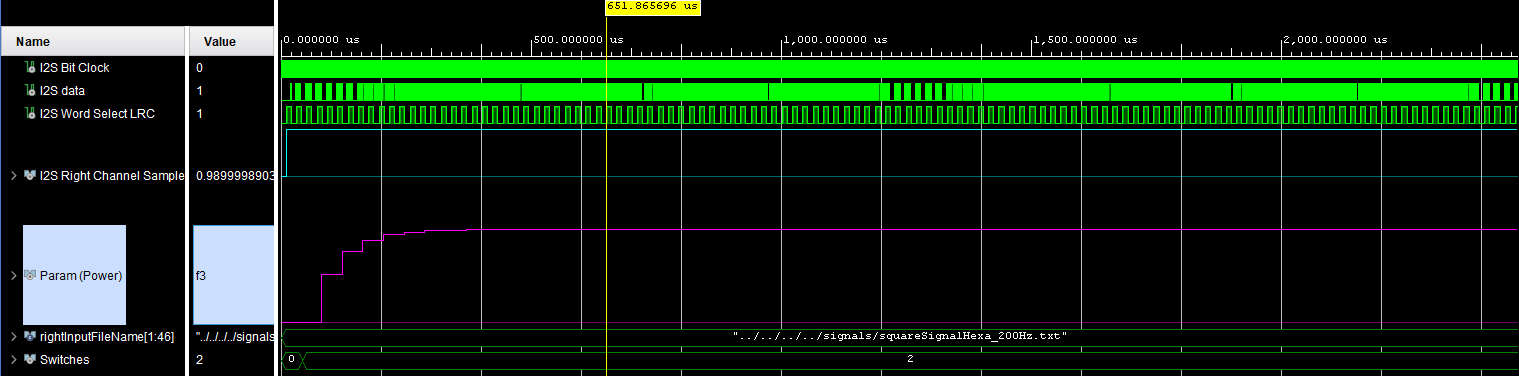
\includegraphics[width=\textwidth]{figures/chrono-m6-saturation-works.png}
    \caption{Saturation du module}
    \label{fig:chrono-m6-saturation-works}
  \end{subfigure}
  \begin{subfigure}{.496\linewidth}
    \centering
    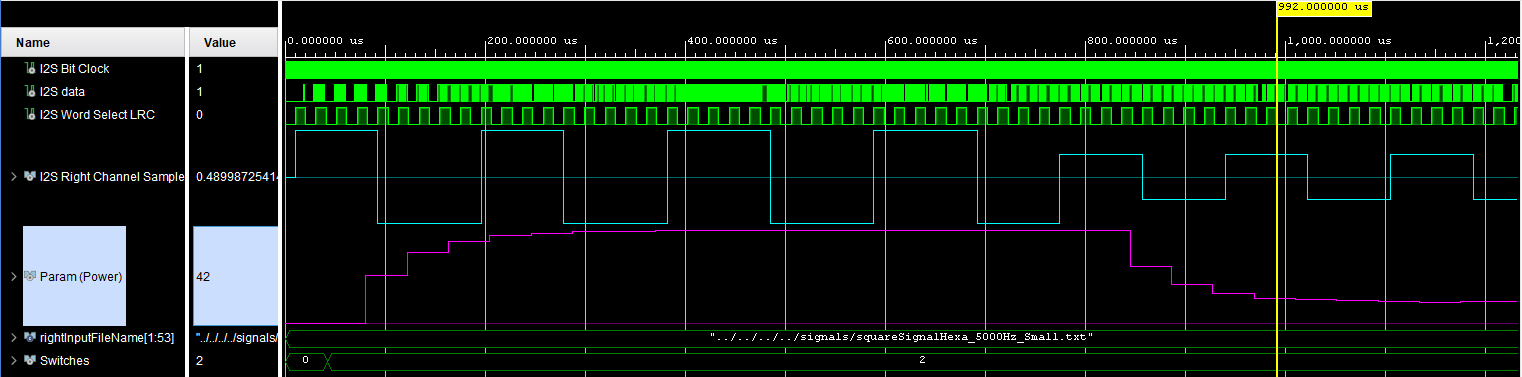
\includegraphics[width=\textwidth]{figures/chrono-m6-square-5000hz-2in1.png}
    \caption{Signal carré à 5000 Hz avec deux canaux}
    \label{fig:chrono-m6-square-5000hz-2in1}
  \end{subfigure}
  \caption{Chronographes du module M6 sous différentes conditions}
\end{figure}

<<<<<<< HEAD
||||||| aa5fd9b
% \quickfigure{Machine à états finis du module M6}{mef-m6}{}{figures/m6-mef-mermaid.pdf}

\todo{Schéma-bloc du système}

\subsection{Description du fonctionnement}

Le module M6 effectue une estimation de la puissance du signal audio en
appliquant un filtrage exponentiel à moyenne glissante sur les échantillons
entrants. Le calcul s'effectue à chaque front montant de l'horloge
\verb|i_bclk|, lorsque le signal \verb|i_en| est à 1. \\

À chaque activation, la puissance instantanée est calculée en élevant au
carré l'échantillon courant \verb|i_ech|. Cette nouvelle valeur est ensuite
ajoutée à l'historique de puissance, qui est préalablement réduite par un
facteur d'oubli de 31/32. Ce facteur assure que les résultats récents ont
plus de poids que les anciens, tout en limitant la croissance de la valeur
accumulée afin d'éviter un débordement (\emph{overflow}). \\

Le résultat final est stocké dans le registre \verb|oldest_power|. Pour
simplifier l'affichage ou l'utilisation de cette puissance, seuls les bits de
poids fort (\verb|oldest_power(46 downto 39)|) sont extraits et envoyés sur
la sortie \verb|o_param|. \\

Le fonctionnement réponds plus ou moins aux spécifications.
À cause de la méthode utilisé, la mesure de la puissance ne se stabilise pas assez lentement pour donner un nombre fixes
à des basses fréquences (\ref{fig:chrono-m6-1000hz-sin-noisy}). Cependant ce chronogramme démontre la résistance au bruit.
La figure \ref{fig:chrono-m6-reset-and-20000hz} démontre le bon fonctionnement du reset (le tout reste à zéro jusqu’à la relâche du signal en rouge).
La figure \ref{fig:chrono-m6-saturation-works} démontre que le calcul monte tranquillement vers le maximum (prouvant l'utilisation d'accumulation)
et n'éprouve aucun dépassement restant stable. la figure \ref{fig:chrono-m6-square-5000hz-2in1} démontre que la puissance reste stable et s'adapte
aux changements d'amplitude du signal entrant dans le module. le chronogramme \ref{fig:chrono-m6-reset-and-20000hz} à une sinus à l'entrée, mais le graphique
à été réalisé avec la fonction d'affichage « hold » se qui donne l'impression d'une onde carré. Les spécification sont
donc atteinte car un facteur de 31/32 est utilisée et une accumulation en continue est présente. Cependant, l'angle d'approche
serait à revoir afin d'avoir des lectures stables avec des ondes sinusoïdales.

=======
% \quickfigure{Machine à états finis du module M6}{mef-m6}{}{figures/m6-mef-mermaid.pdf}

\todo{Schéma-bloc du système}

\subsection{Description du fonctionnement}

Le module M6 effectue une estimation de la puissance du signal audio en
appliquant un filtrage exponentiel à moyenne glissante sur les échantillons
entrants. Le calcul s'effectue à chaque front montant de l'horloge
\verb|i_bclk|, lorsque le signal \verb|i_en| est à 1. \\

À chaque activation, la puissance instantanée est calculée en élevant au
carré l'échantillon courant \verb|i_ech|. Cette nouvelle valeur est ensuite
ajoutée à l'historique de puissance, qui est préalablement réduite par un
facteur d'oubli de 31/32. Ce facteur assure que les résultats récents ont
plus de poids que les anciens, tout en limitant la croissance de la valeur
accumulée afin d'éviter un débordement (\emph{overflow}). \\

Le résultat final est stocké dans le registre \verb|oldest_power|. Pour
simplifier l'affichage ou l'utilisation de cette puissance, seuls les bits de
poids fort (\verb|oldest_power(46 downto 39)|) sont extraits et envoyés sur
la sortie \verb|o_param|. \\

Le fonctionnement réponds plus ou moins aux spécifications.
À cause de la méthode utilisé, la mesure de la puissance ne se stabilise pas assez lentement pour donner un nombre fixes
à des basses fréquences (chronogramme A \ref{fig:chrono-m6-1000hz-sin-noisy}). Cependant ce chronogramme démontre la résistance au bruit.
La figure \ref{fig:chrono-m6-reset-and-20000hz} démontre le bon fonctionnement du reset (le tout reste à zéro jusqu’à la relâche du signal en rouge).
La figure \ref{fig:chrono-m6-saturation-works} démontre que le calcul monte tranquillement vers le maximum (prouvant l'utilisation d'accumulation)
et n'éprouve aucun dépassement restant stable. la figure \ref{fig:chrono-m6-square-5000hz-2in1} démontre que la puissance reste stable et s'adapte
aux changements d'amplitude du signal entrant dans le module. le chronogramme \ref{fig:chrono-m6-reset-and-20000hz} à une sinus à l'entrée, mais le graphique
à été réalisé avec la fonction d'affichage « hold » se qui donne l'impression d'une onde carré. Les spécification sont
donc atteinte car un facteur de 31/32 est utilisée et une accumulation en continue est présente. Cependant, l'angle d'approche
serait à revoir afin d'avoir des lectures stables avec des ondes sinusoïdales.

>>>>>>> f3a95d1f7e042059d91cdd06ce5bf5d9d6d49af1
% \todo{Description sommaire du fonctionnement}
%\todo{Plan de vérification}

%\todo{Validation via une simulation avec le banc de test fourni. Vous devez démontrer le
%fonctionnement de vos modules au travers de simulations et expliquez en quoi vous
%répondez aux spécifications. Faites bon usage des curseurs, formattage des données et
%agrandissements pour appuyer vos propos.}


\section{Conclusion}

Au terme de ce projet, nous avons conçu, implémenté et vérifié quatres modules dont deux sont présentés dans ce rapport pour le traitement audio numérique sur FPGA, soit le décodeur I2S (M1) et le calculateur de puissance (M6). Le module M1 a démontré une désérialisation fiable des échantillons audio stéréo, tout en respectant la synchronisation imposée par le protocole I2S. Quant au module M6, il a permis une estimation continue de la puissance du signal en intégrant une stratégie de filtrage efficace, bien que perfectible à basse fréquence.

Les résultats obtenus à travers les plans de vérification et les simulations confirment la fonctionnalité attendue de chacun des modules selon les critères du projet. Ce travail a permis de consolider nos compétences en conception VHDL, en validation de systèmes logiques, ainsi qu’en méthodologie de développement modulaire sur FPGA.

\end{document}
